\documentclass{article}
\usepackage{amsmath}
\usepackage{geometry}
\usepackage{graphicx}
\usepackage{caption}
\usepackage{url}
\usepackage{subcaption}
\usepackage{minted}
\captionsetup{labelformat = empty}
\renewcommand{\contentsname}{Innholdsfortegnelse}
\geometry{a4paper, margin=3cm}

\begin{document}

\begin{titlepage}
    \begin{minipage}{0.3\textwidth}
        
\includegraphics[width=2.5cm]{Elsyslogo.png}
    \end{minipage}
    \hfill
    \begin{minipage}{0.65\textwidth}
        \raggedright
        \LARGE \textbf{Sluttrapport – "Nomes Kopp"} \\[1em]
        \large Albert Waagaard Fougner \\ Ask Moen Kobbenes \\ Isak Brevik \\ Jacob Halsne Berentsen \\ Vetle Mathias Botten \\ Sølve Brun Kjelstrup \\ Tobias Duna Lundemo \\[1em]
        \normalsize 01.11.2024
    \end{minipage}
    \vfill
    \begin{center}
        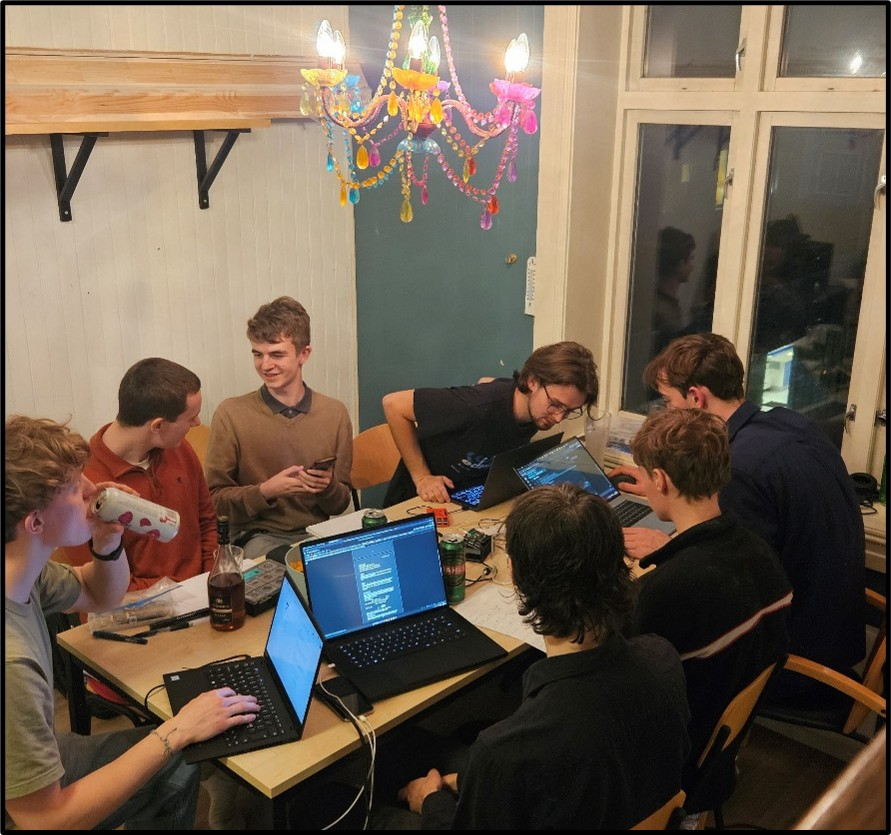
\includegraphics[width=10cm]{Gruppebilde1.jpg}
    \end{center}
\end{titlepage}
\newpage
\tableofcontents{}

\section{Problemstilling}
\label{Problemstilling}
Da jeg fikk dette prosjektet, tenkte jeg slik:\\
Det er tre ting jeg elsker – matte, elektronikk og en god øl.  
Det er tre ting jeg ikke kan fordra – god øl som har blitt varm, vektorrom og packet loss.

\section{Konsept}
\label{Konsept}
Dermed samlet jeg mine beste kompiser fra studiet, kjøpte mye øl, diverse elektroniske komponenter og satte i gang prosjektet.  
Målet vårt: en kopp som regner ut hvor lang tid jeg har på å drikke ølen min før den blir varm.

\section{Design}
\label{Design}
``A \textbf{cup} is an open-top container used to hold liquids for \textbf{pouring} or \textbf{drinking}.''\footnote{\url{https://en.wikipedia.org/wiki/Design_principles}}\footnote{\url{https://en.wikipedia.org/wiki/Mug}}
\vfill
\begin{center}
    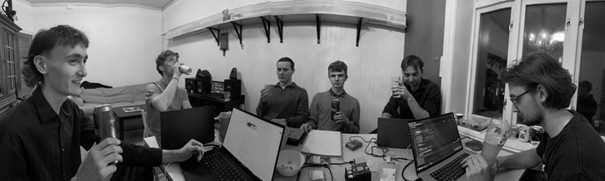
\includegraphics[width=\textwidth]{Panorama_pilsing.jpg}
\end{center}
\newpage
\section{Implementering}
\label{Implementering}
\subsection{Metode}
\label{Metode}
Prosjektet løser jeg smertefritt ved å smelle sammen en ESP-32, en Raspberry Pi og et par temperatursensorer. Essensen i kodene følger.
Newtons avkjølingslov,
\[ 
\frac{dT_{\text{øl}}}{dt} = -\alpha(T_{\text{øl}} - T_{\text{omg}})
\]
der
\[ 
T_{\text{øl}}(0) = T_{0}
\]
gir
\[ 
T_{\text{øl}} = T_{\text{omg}} + (T_{0} - T_{\text{omg}})e^{-\alpha t}
\]
Denne difflikningen løste jeg heldigvis i barnehagen.
Løser videre for \(t\):
\[ 
t = -\frac{1}{\alpha} \ln \left(\frac{T_{0} - T_{\text{omg}}}{T_{\text{øl}} - T_{\text{omg}}}\right)
\]
hvor \(t\) er tiden mellom \(T(0)\) og aktuell tid. Jeg har nå løst for kjente temperaturverdier, og setter da resultatet tilbake i originaluttrykket. Herifra kan vi finne ut hvor lang tid (\(t\)) det vil ta før ølen blir for varm, eksempelvis ved å sette 14 °C som grensen for temperatur for \(T_{\text{t}}\) (uff, det er altfor varmt øl) og bytte \(T(0)\) med den nåværende temperaturen.\\
\subsection{Realisering}
\label{Realisering}
Jeg koblet så sammen et breadboard med luft- og væsketemperatursensorer, og en ESP-32, og startet programmeringen.
Jeg lagde først et enkelt program for ESP-32 som sender temperaturen over seriell kommunikasjon videre til et pythonprogram som lagrer tid, temperatur i øl, og temperatur lufta i et tekstdokument. Deretter lagde jeg et nytt program som plottet dataen, sammen med den teoretiske kurven for temperaturedringen.
Etter litt testing for å kontrollere at systemet fungerer, la jeg til den ønskede funksjonaliteten; Beregning av tiden jeg har på meg til å drikke ølen min, gjort direkte på ESP'en, og printing av tiden til en liten OLED-skjerm.
\vfill
\begin{center}
    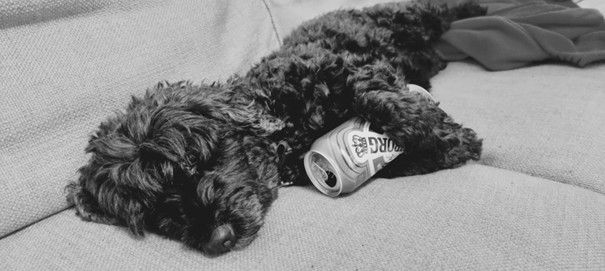
\includegraphics[width=15cm]{Tinka_med_pils.jpg}
\end{center}
\newpage

\section{Verifikasjon og test}
\label{Verifikasjon og test}
For de innledende testene av systemet, klarte jeg ikke å få meg selv til å bruke øl og sløse de edle dråpene, da et slikt alkoholmisbruk ikke er en masterstudent verdig. Da ble det kaldt vann fra springen.
Som vi ser fra Figur \ref{fig:temperaturgraf}, har det vært sterkt varierende lufttemperatur på en dårlig isolert hytte under denne testen. Jeg har i Figur \ref{fig:glattet} glattet ut kurven med litt enkel kode. Etter denne testen, med en så fin graf, er jeg trygg på at koden min fungerer og at jeg kan fortsette.
\begin{figure}[h!]
    \centering
    \begin{subfigure}[b]{0.45\textwidth}
        \centering
        \includegraphics[width=\textwidth]{Rå_data.png}
        \caption{Temperaturgraf}
        \label{fig:temperaturgraf}
    \end{subfigure}
    \hfill
    \begin{subfigure}[b]{0.45\textwidth}
        \centering
        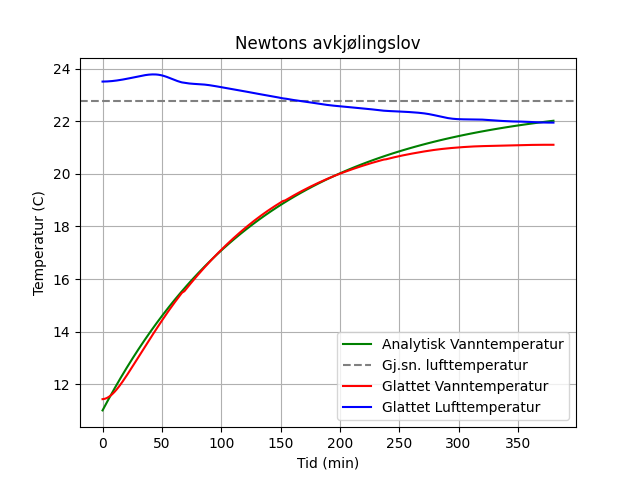
\includegraphics[width=\textwidth]{Glattet_data.png}
        \caption{Glattet data}
        \label{fig:glattet}
    \end{subfigure}
    \caption{Sammenligning av rådata og glattet data}
\end{figure}\\
Etter en test med vann var jeg klar for å teste systemet mitt med øl. Jeg jekket en nydelig dahls pils og helte den i glasset, lå temperatursensoren nedi og startet ESP'en. Etter ett minutt, og to målinger, har koden beregnet antatt tid til ølet mitt er for varmt. Den påsto at det ville ta 47 minutter, og for vitenskapens skyld bestemte jeg meg for å se om det stemte. Jeg startet nedtelling, og om vi ser fra Figur \ref{fig:tid_sammenlikn} stemte matematikkens prediksjoner av virkeligheten rimelig godt. Faktisk var feilberegningen bare på snaue 10 sekunder! Dette var godt nok for oss. Den beregnede temperaturkonstanten, alpha, ble i vårt forsøk ca. 0.0096.
\newline
\begin{figure}[h!]
    \centering
    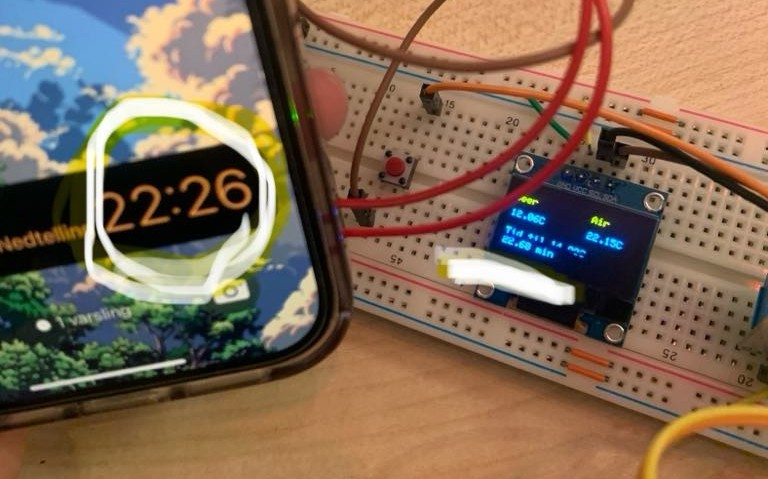
\includegraphics[width=0.7\linewidth]{tid_sammenlikning.jpg}
    \caption{Sammenlikning av beregnet tid}
    \label{fig:tid_sammenlikn}
\end{figure}
\newpage
\begin{figure}[h!]
    \centering
    \begin{subfigure}[b]{0.45\textwidth}
       \centering
        \includegraphics[width=\textwidth]{Rå_data_2.png}
        \caption{Øltemperatur}
        \label{fig:dahls_test}
    \end{subfigure}
    \hfill
    \begin{subfigure}[b]{0.45\textwidth}
        \centering
        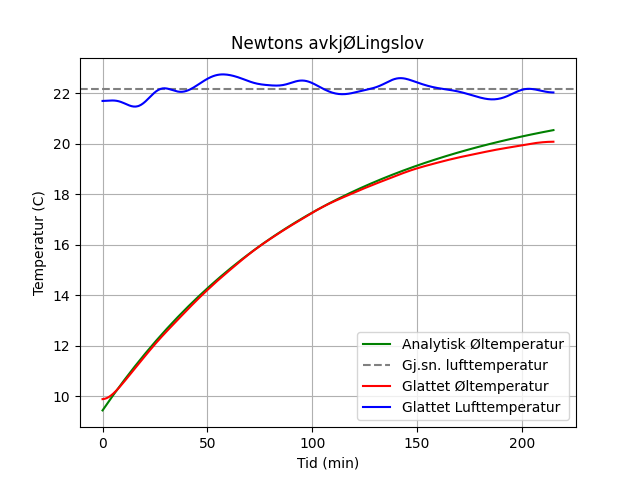
\includegraphics[width=\textwidth]{Glattet_data_2.png}
        \caption{Utgjevnet kurve}
        \label{fig:glattet_dahls}
    \end{subfigure}
    \caption{Endelig test}
\end{figure}
\vfill
\begin{figure}[h!]
    \centering
    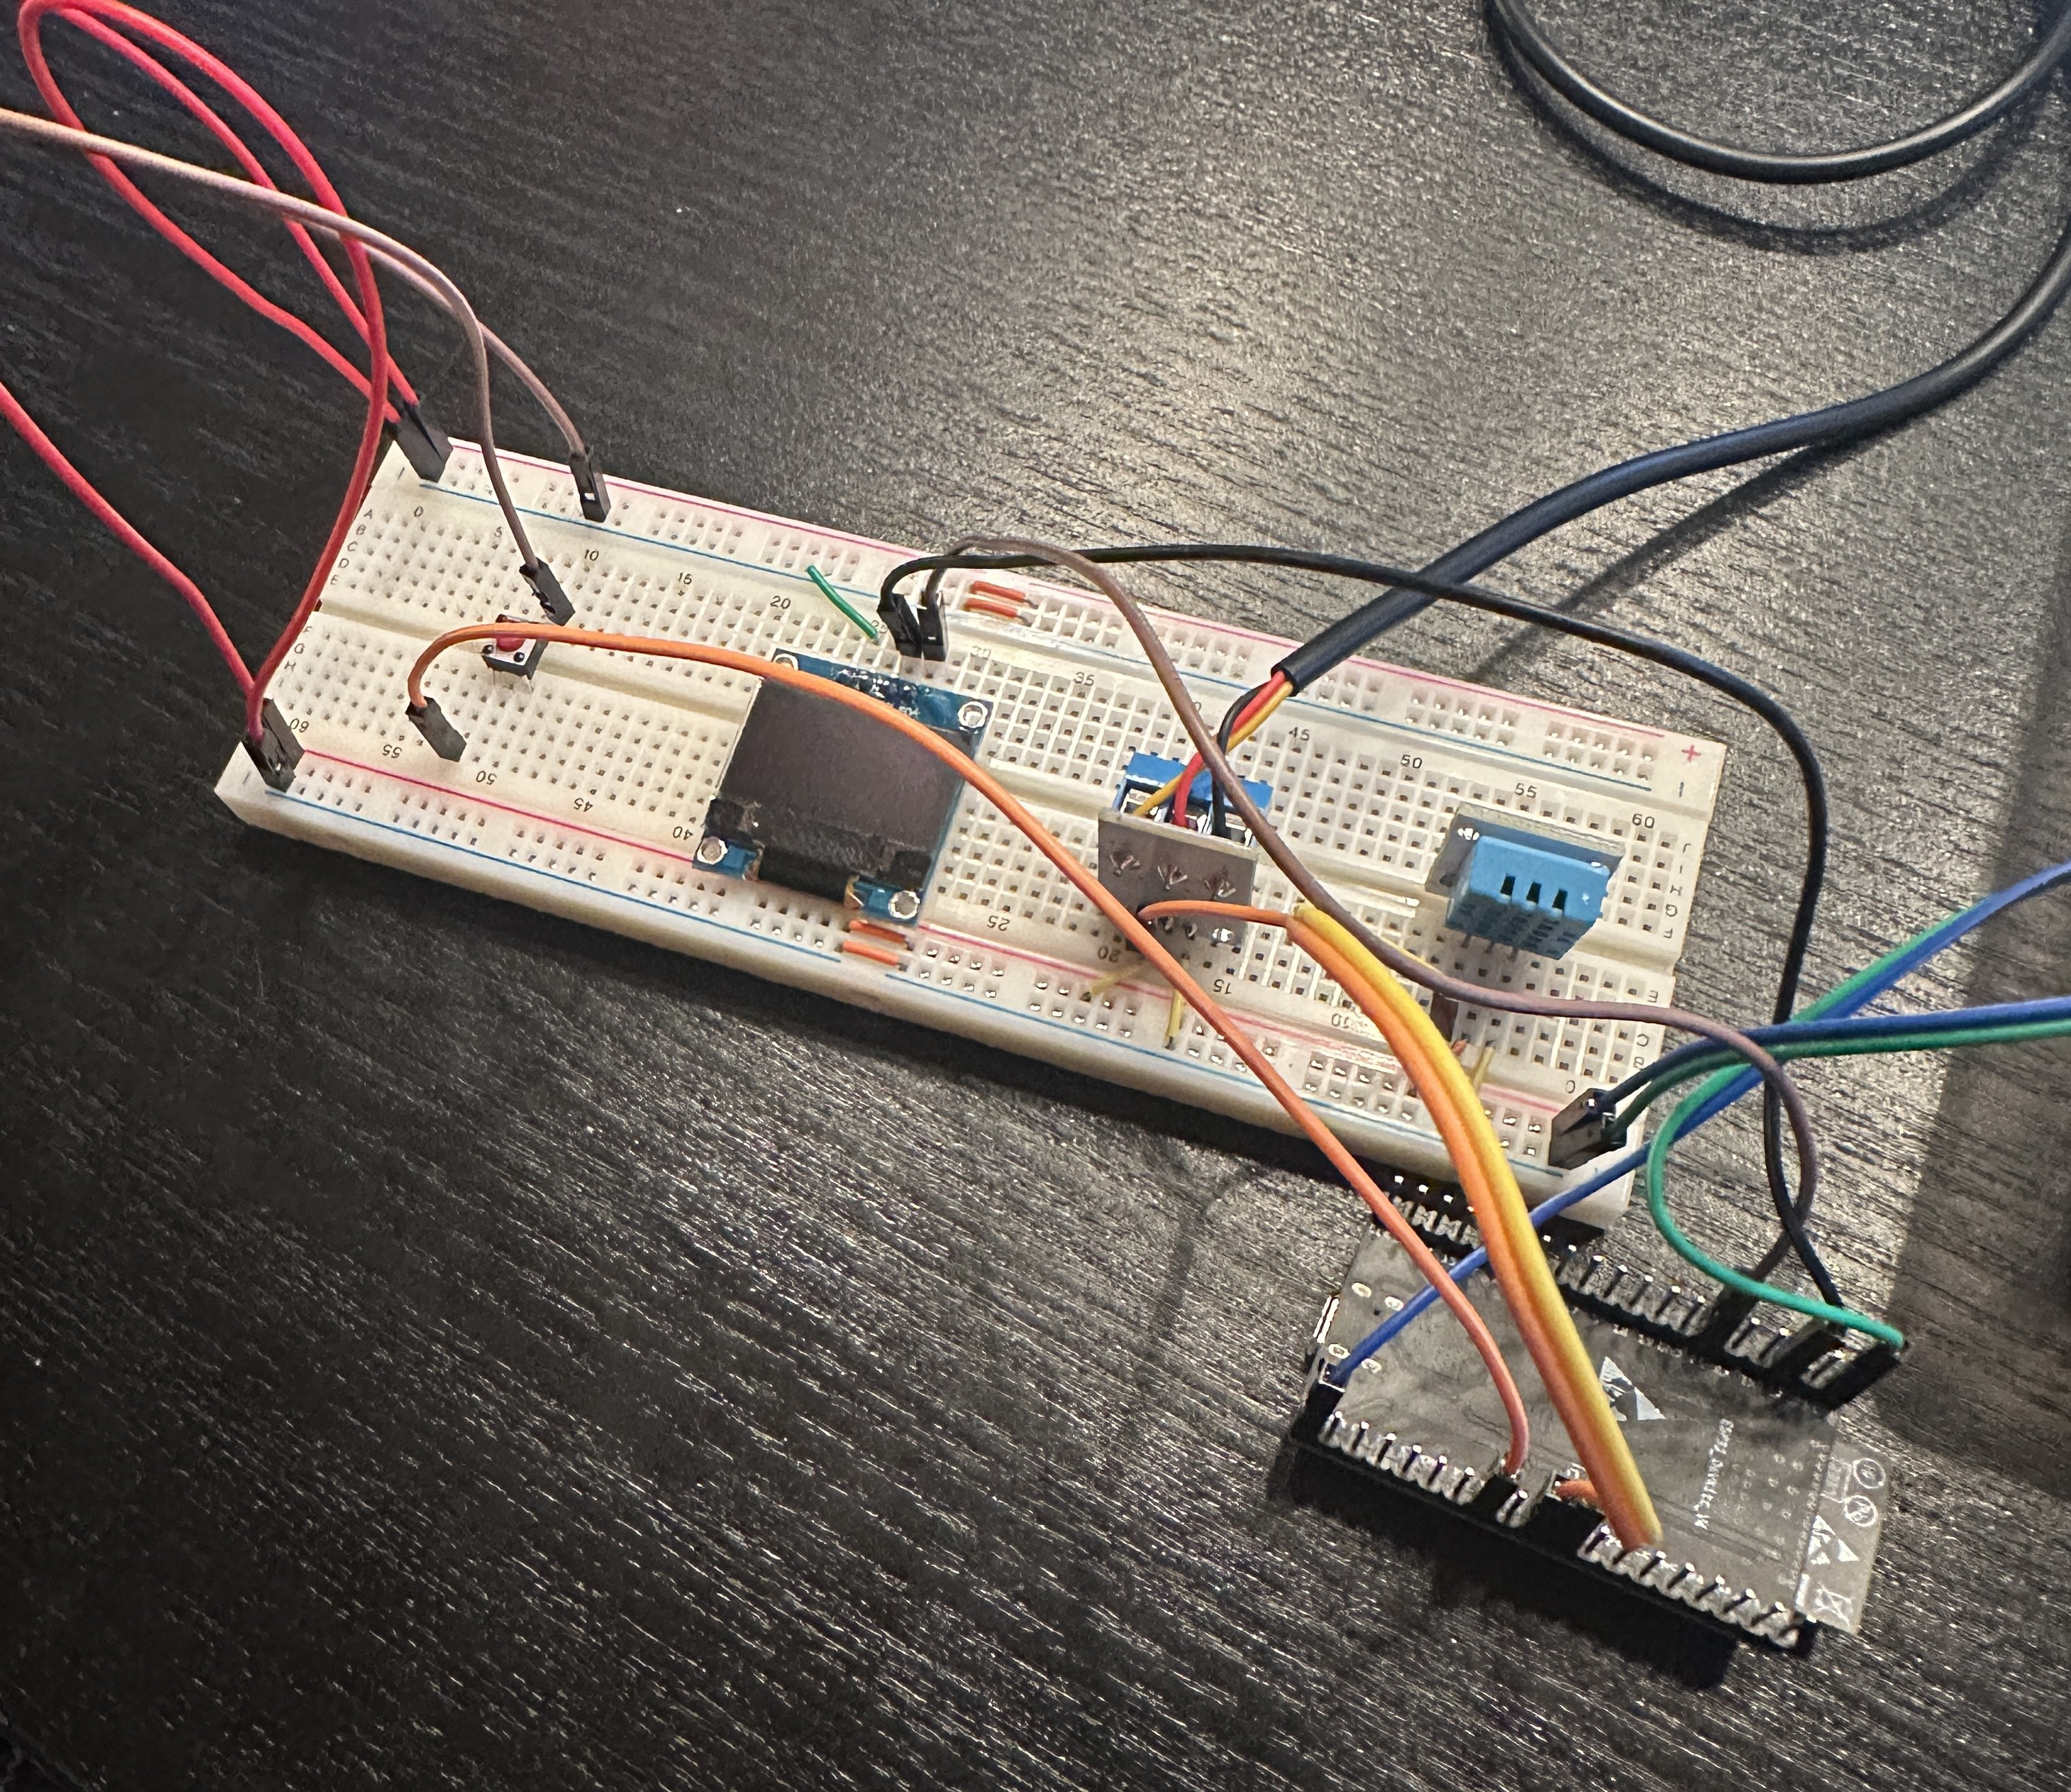
\includegraphics[width=0.8\linewidth]{Oppkobling.JPEG}
    \caption{Bilde av oppkoblingen}
    \label{fig:oppkobling}
\end{figure}
\newpage
\section{Kode}
\label{Kode}
All kode kan all kode kan hentes på github, se vedlegg \ref{github}.
\subsection{Arduino-kode (C++)}
\label{C++}
\begin{minted}{C++}
// Funksjon for å beregne tiden til øltemperaturen når targetTemp
float beregnTidTilMålTemp(float T_0, float T_k, float T_mål, float alpha) {
  return -log((T_mål - T_k) / (T_0 - T_k)) / alpha;
}
// Sjekk om temperaturen vil stige eller synke
if ((første_øltemp - lufttemp) != 0) {
    // Beregn alpha kontinuerlig basert på første og nyeste måling
    alpha = -log(fabs((øltemp - lufttemp) / (første_øltemp - lufttemp))) 
    / ((millis() / 60000.0) - starttid);
    }

// Beregn forventet tid til måltemperatur med kontinuerlig alpha
float tidTilMålTemp = beregnTidTilMålTemp(øltemp, lufttemp, targetTemp, alpha);

\end{minted}
Denne delen av koden beregner proporsjonalitetskonstanten kontinuerlig, og oppdaterer forventet tid til temperaturgrensen. Etter denne beregningen printes resultatet til skjerm som vist i Figur \ref{fig:tid_sammenlikn}.
I tillegg til printing til skjerm, printes tiden etter start og temperaturene til seriell kommunikasjon med denne kodesnutten:
\begin{minted}{C++}
// Print til seriell for logging
Serial.print((millis() / 60000.0) - starttid);
Serial.print(',');
Serial.print(øltemp);
Serial.print(',');
Serial.println(lufttemp);
\end{minted}
\begin{center}
    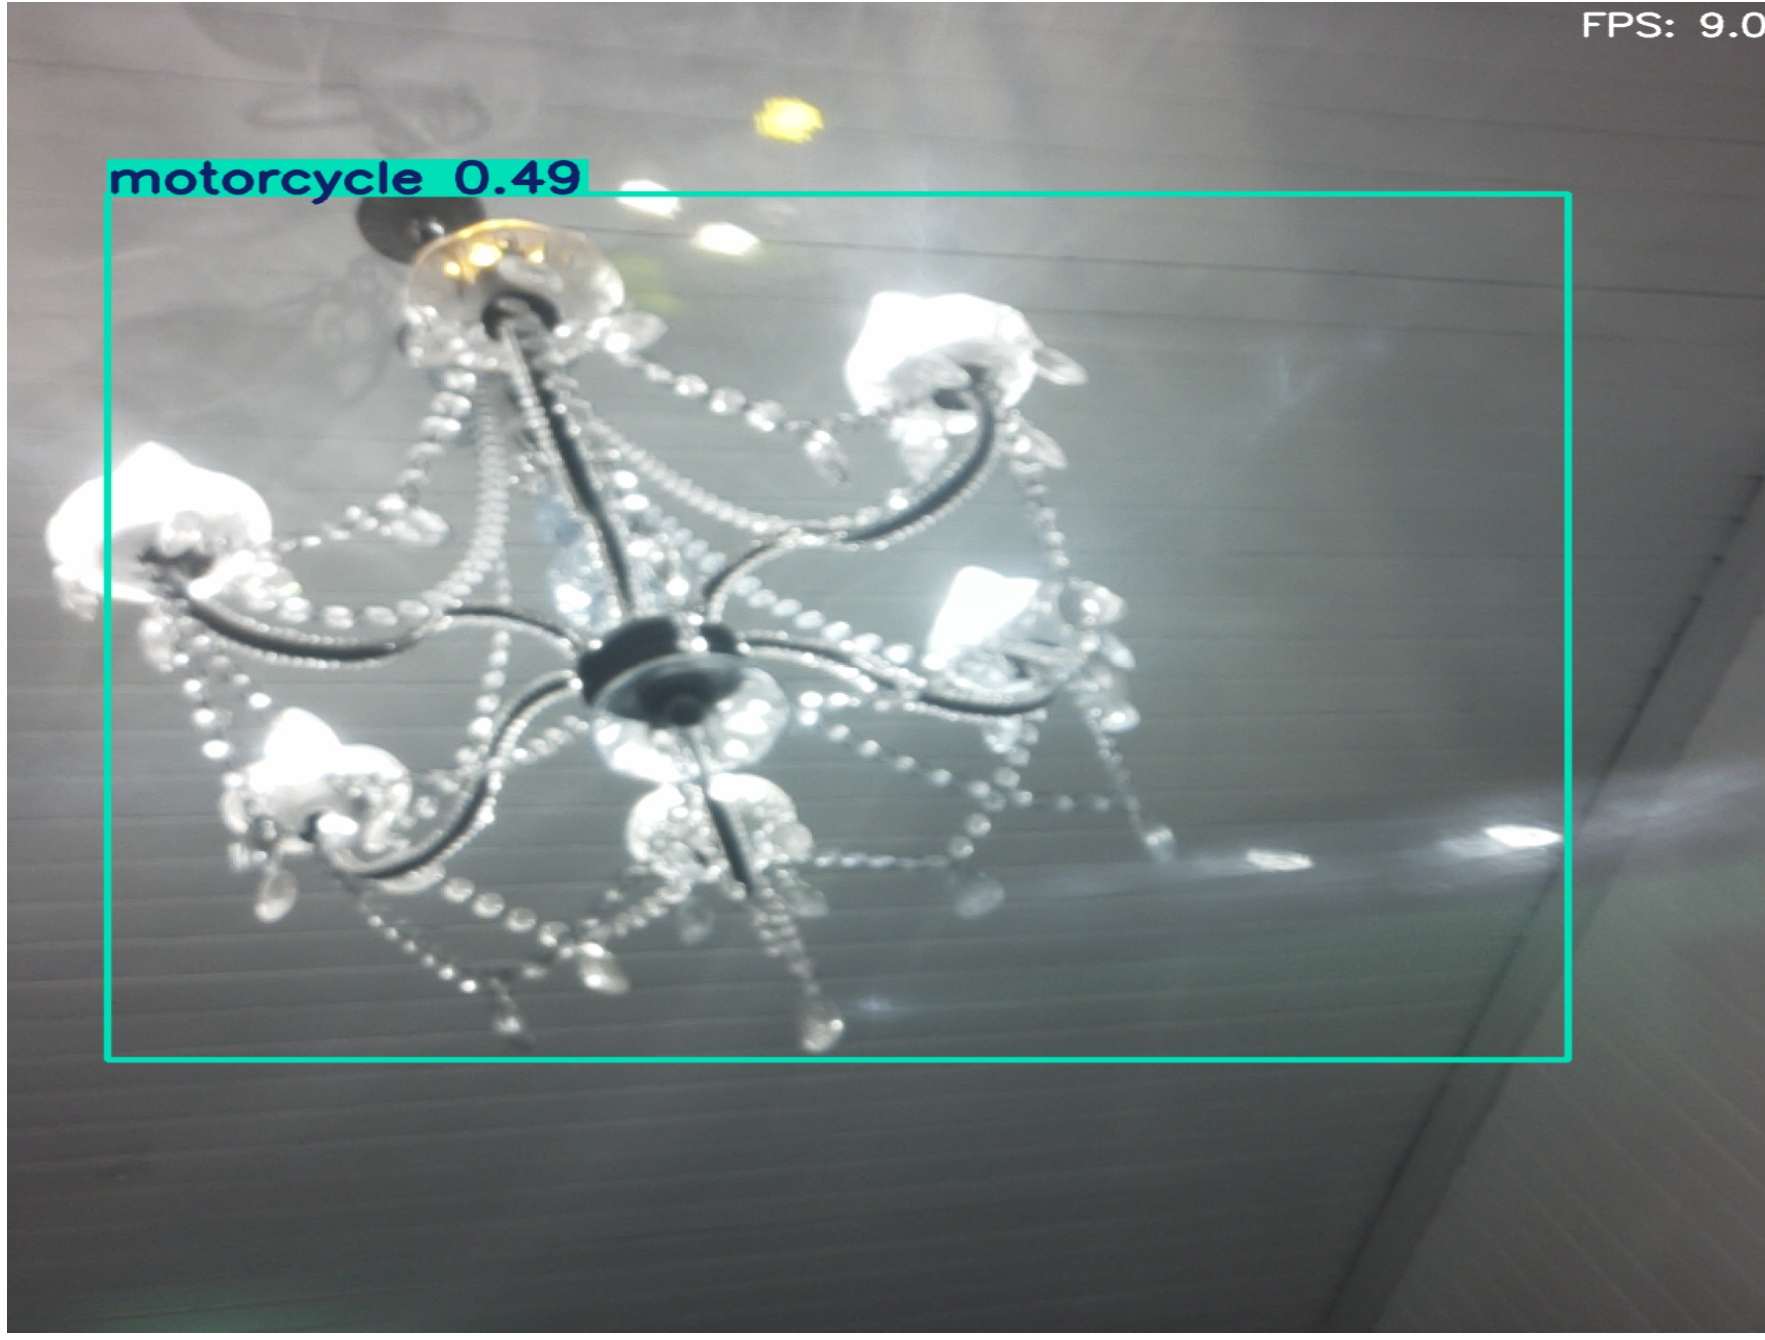
\includegraphics[width=0.8\linewidth]{motorcycle.png}\footnote{Var ikke like stor suksess for ELSYSGK prosjektet mens vi ventet på varmt øl}
\end{center}
\vfill
\subsection{Python-kode}
\label{Python}
Python-koden for loggføring av temperatur:
\begin{minted}{python}
import serial
import time

# Konfigurer seriell port
ser = serial.Serial('COM3', 115200)
tid_før = time.perf_counter()
# Åpne fil for å lagre data
with open("temp_log.txt", "w") as file:
    file.write("Tid, Temp \n")

    while time.perf_counter() - tid_før < 15000:
        if ser.in_waiting > 0:
            data = ser.readline().decode().strip()
            print(data)
            file.write(str(data) + '\n' )
            file.flush()
ser.close()
\end{minted}
Essensen i python-koden for plottingen er som følger;\\
Definisjon av den analytiske løsningsfunksjonen for newtons avkjølingslov:
\begin{minted}{python}
def analytisk_løsning(t, T_0, alpha, T_k):
    return T_k + (T_0 - T_k) * np.exp(-alpha * t)
\end{minted}
Beregning av proporsjonalitetskonstanten:
\begin{minted}{python}
    dT_0 = T_0 - T_k
    dT_1 = T_1 - T_k
    alpha = -np.log(dT_1 / dT_0) / dt
\end{minted}
Funksjon for plotting av teoretisk temperaturendring:
\begin{minted}{python}
def plot_newtons_avkjøling(T_0, T_1, T_k, tid, dt): 
    [...]
    T = analytisk_løsning(t, T_0, alpha, T_k)
    plt.plot(t, T, label="Analytisk Vann/øltemperatur", color="green")
    plt.axhline(T_k, color='gray', linestyle='--', label=f"Gj.sn. lufttemperatur")
    [...]
\end{minted}

\section{Konklusjon}
\label{Konklusjon}
Jeg kan fint konkludere med at jeg, og gruppen, har oppnådd målet. Nå kan jeg trygt sette fra meg ølen min, uten å være redd for at den blir varm.
\vfill
DISCLAIMER: intet øl gikk til spille under prosjektet

\begin{center}
    
\includegraphics{GPT_math_joke.png}
\end{center}

\appendix
\small \section{Link til github}
\label{github}
\textbf{\url{https://github.com/TobiasDuna/pub/tree/main/matte_oblig_2024}}

\end{document}
\section*{Referanser}
Forfatter, Tittel, Utgiverinformasjon, år. \\
Forfatter, Tittel, Utgiverinformasjon, år.